\section*{Assignment 01: Platform Concept and Value Proposition}
\addcontentsline{toc}{section}{Assignment 01: Platform Concept and Value Proposition}

The platform concept I develop, \textbf{SkillSync}, imagines a bridge between students chasing real projects and small organisations that need help but lack consultant budgets. SkillSync would act as digital infrastructure facilitating repeated exchanges between distinct user groups \citep{Choudary2016}. The core promise is a scoped collaboration that gives students portfolio wins while NGOs unlock motivated talent for a few intense weeks.

The concept only clicked after several quiet iterations. Early notes just said ``students helping real-world actors,'' which felt like a slogan more than a design. Guided by \citet{Choudary2016} and \citet{Srnicek2017} I tightened the idea into a project-based platform that sits between internships and gig work: flexible enough to dodge HR red tape yet structured enough to deliver measurable outcomes once it exists.

SkillSync therefore behaves, in theory, as a two-sided orchestrator. Students would bring skills and energy; NGOs and civic teams would bring real problems. The design emphasises trustworthy matchmaking so cross-side network effects can blossom. Institutional email verification, lightweight vetting, and a templated scoping wizard sit on the draft checklist to keep expectations aligned before anyone spends serious time, echoing the launch hygiene emphasised in Lecture~2 on platform network effects \citep{Lecture02}.

Data is the quiet engine in the imagined operating model. Each project could generate feedback, endorsements, and behavioural signals. In the short run, that data would refine matching; in the longer run, it could craft portable skill passports, nodding to the credentialing space \citet{Zuboff2019} critiques. The value proposition therefore lives inside those loops as much as in the pitch deck.

Figure~\ref{fig:student-view} renders the promise as a mock-up. The sketched student dashboard highlights curated projects while pinning progress nudges and mentor notes on the right. Project cards emphasise stipend range, time commitment, and deliverables because uncertainty kills motivation, and the ``mentor check-in'' strip imagines past data keeping guidance personal.

\begin{figure}[H]
  \centering
  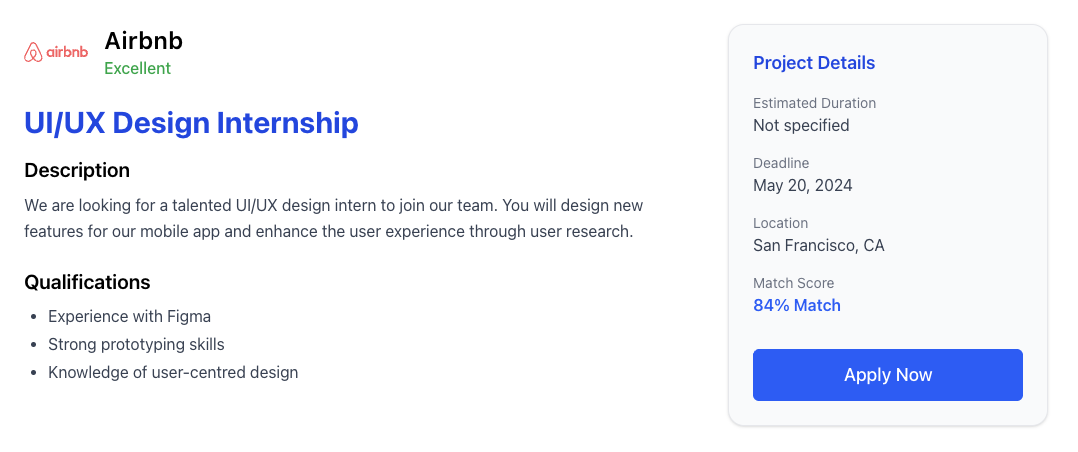
\includegraphics[width=0.85\linewidth]{figures/Student-Project-View.png}
  \caption{Student project workspace mock-up with progress nudges.}
  \label{fig:student-view}
\end{figure}

On the supply side, I mirror the experience for NGOs. The creation wizard walks through a scoping checklist in plain language: desired outcome, must-have skills, support on offer. Desk research suggests such a template could be completed within minutes. The figure in Assignment~3 shows that workflow in action. The value proposition is therefore more than a slogan about ``students meet projects''; it is a set of proposed micro-interactions that reduce uncertainty for both sides and make repeat usage more likely.
